\section{Zukünftige Ergänzungen} \label{sec:praktischeUmsetzung:ausblick}
Abschließend soll auf zwei Anforderungen eingegangen werden, die noch nicht umgesetzt oder getestet wurden, weil das Bestandssystem diese nicht erfüllt und sie damit für den Migrationsprozess nicht relevant sind.

\subsection{Auswertung von Personendaten}
Aufgrund des neuen Self-Service Reportings mit \textit{Power BI} wird vermutet, dass das Interesse an individuellen Auswertungen zukünftig steigen wird. Die Auswertung der erbrachten Leistungen einzelner Personen ist aus regulatorischen Gründen ein schwieriges Thema und erfordert die Zustimmung des Betriebsrates. Für die meisten Benutzer könnte dies über eine Gruppe mit entsprechenden Rechten im \ac{aad} gelöst werden, in der die Mitglieder vom Betriebsrat verwaltet werden. Datenbankadministratoren hätten jedoch immer noch die Möglichkeit, auf die Personendaten zuzugreifen. Mit der Datenbankfunktion \textit{Always Encrypted} kann das verhindert werden. \textit{Always Encrypted} ermöglicht es Spalten zu verschlüsseln und kann damit auch Datenbankadministratoren daran hindern sensitive Daten zu lesen. Der verwendete Schlüssel wird im \textit{Key Vault} gespeichert und die dort eingestellten Zugriffsberechtigungen auf den Schlüssel, bestimmen, wer die Daten unverschlüsselt abfragen kann. Die Entschlüsselung während der Abfrage passiert dabei automatisch \cite{mauri_practical_2021}. Es wäre demnach ausreichend, der zuvor erstellten Gruppe, Zugriff auf den Schlüssel im \textit{Key Vault} zu gewähren. Einem Datenbankadministrator, der nicht in dieser Gruppe ist, werden dann nur verschlüsselte Binärwerte angezeigt und er kann keine Auswertungen durchführen.

\subsection{Machine Learning für fortgeschrittene Analysen}
\label{sec:praktischeUmsetzung:ausblick:aml}
Beim Entwurf der neuen Architektur wurde bereits die Möglichkeit berücksichtigt, das BI-System um Machine Learning Funktionalitäten zu ergänzen. Dafür wird der Dienst \ac{aml} vorgesehen, mit dem fortgeschrittene Analysen mit Python und R möglich sind. Abbildung~\ref{fig:praktischeUmsetzung:ausblick:aml} zeigt auf Basis des vereinfachten Konzepts (siehe Abbildung~\ref{fig:chap03_4_konzeptArchitektur_offen}), wie die zukünftige Intgration von \ac{aml} aussehen könnte.

\begin{figure}[htbp]
 \centering
 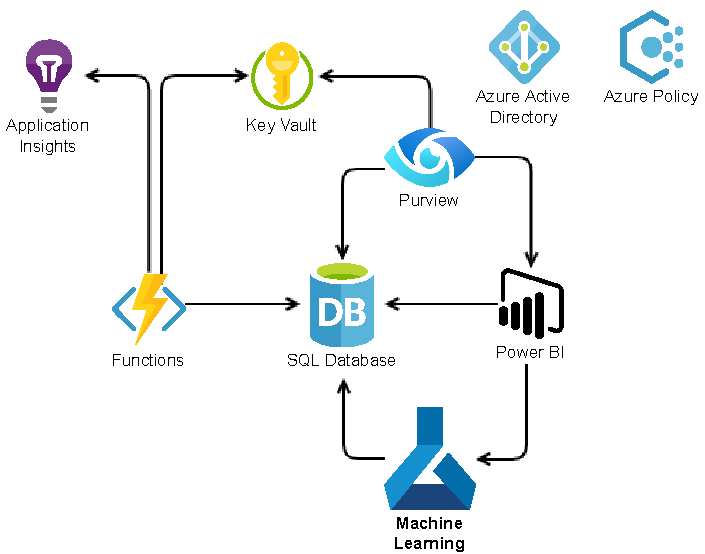
\includegraphics[width=0.7\textwidth]{gfx/azure/aml.pdf}
 \caption[Vereinfachtes Konzept für Azure BI-Architektur mit Machine Learning]{Vereinfachtes Konzept für Azure BI-Architektur mit \textit{Machine Learning}}
\label{fig:praktischeUmsetzung:ausblick:aml}
\end{figure}

Bei dem gezeigten Konzept wird von den Funktionalitäten, die bereits bei der Vorstellung von \ac{aml} in Abschnitt~\ref{sec:grundlagen:azure_dienste:machineLearning} beschrieben wurden, ausgegangen. Das bedeutet, dass \ac{aml} Zugriff auf das \ac{dwh} erhalten muss, damit die Daten für die verschiedenen Machine Learning Prozesse zugänglich gemacht werden können. Für \textit{Power BI} werden Webendpunkten in \ac{aml} bereitgestellt, wodurch die fortgeschrittene Analysen im Reporting genutzt werden können. \cite[vgl.][]{soh_data_2020}